\documentclass[12pt, a4paper]{article}
\usepackage[utf8]{inputenc}
\usepackage{graphicx}
\usepackage{geometry}
\usepackage{hyperref}
\usepackage{listings}
\usepackage{xcolor}
\usepackage{tikz}
\usetikzlibrary{shapes.geometric, arrows, positioning}
\usepackage{float}
\usepackage{caption}
\usepackage{subcaption}

\geometry{margin=1in}

% Colors for code listings
\definecolor{codegreen}{rgb}{0,0.6,0}
\definecolor{codegray}{rgb}{0.5,0.5,0.5}
\definecolor{codepurple}{rgb}{0.58,0,0.82}
\definecolor{backcolour}{rgb}{0.95,0.95,0.92}

\lstdefinestyle{mystyle}{
    backgroundcolor=\color{backcolour},   
    commentstyle=\color{codegreen},
    keywordstyle=\color{magenta},
    numberstyle=\tiny\color{codegray},
    stringstyle=\color{codepurple},
    basicstyle=\ttfamily\footnotesize,
    breakatwhitespace=false,         
    breaklines=true,                 
    captionpos=b,                    
    keepspaces=true,                 
    numbers=left,                    
    numbersep=5pt,                  
    showspaces=false,                
    showstringspaces=false,
    showtabs=false,                  
    tabsize=2
}

\lstset{style=mystyle}

\title{\textbf{Shree Anna Connect: AI-Powered Millet Marketplace}\\ \large Comprehensive Project Report & Architectural Analysis}
\author{Development Team}
\date{\today}

\begin{document}

\maketitle

\begin{abstract}
This document provides a comprehensive technical analysis of \textbf{Shree Anna Connect}, a digital marketplace designed to empower millet farmers through advanced Artificial Intelligence. We detail the system architecture, the integration of Google's Gemini models for multimodal capabilities, and the rationale behind our technology choices. We specifically address the efficiency, reliability, and trustworthiness of the Gemini ecosystem in the context of agricultural technology. Finally, we outline the roadmap for future enhancements, including offline capabilities and blockchain integration.
\end{abstract}

\tableofcontents
\newpage

\section{Introduction}
\subsection{Problem Statement}
Millet farmers in India face significant challenges, including:
\begin{itemize}
    \item Lack of real-time market price information, leading to distress selling.
    \item Difficulty in accessing government schemes (e.g., Shree Anna Abhiyan) due to language barriers and complex documentation.
    \item Inability to objectively assess produce quality, resulting in unfair pricing from middlemen.
    \item Limited access to direct buyers (B2B).
\end{itemize}

\subsection{Proposed Solution}
\textbf{Shree Anna Connect} is a holistic platform that bridges the gap between farmers and buyers. It leverages:
\begin{itemize}
    \item \textbf{AI Chatbot}: For instant, multilingual assistance on schemes and farming practices.
    \item \textbf{Computer Vision}: For automated quality grading of millet samples.
    \item \textbf{Predictive Analytics}: For fair price discovery based on market trends.
    \item \textbf{Smart Matching}: To connect farmers directly with institutional buyers.
\end{itemize}

\section{System Architecture}
The system follows a modern \textbf{Microservices Architecture}, ensuring scalability, maintainability, and separation of concerns.

\subsection{Architectural Components}
\begin{enumerate}
    \item \textbf{Frontend (Client Layer)}: Built with \textbf{React (Vite)}, styled with \textbf{Tailwind CSS} and \textbf{Shadcn UI}. It provides a responsive interface for farmers and buyers.
    \item \textbf{Backend (Service Layer)}: A lightweight \textbf{FastAPI} (Python) microservice that handles business logic and orchestrates AI requests.
    \item \textbf{AI Engine (Intelligence Layer)}: Powered by \textbf{Google Gemini 1.5 Flash} and \textbf{Gemini 2.0 Flash} via the Google Generative AI SDK.
    \item \textbf{Database (Data Layer)}: \textbf{Supabase} (PostgreSQL) for persistent storage of user profiles, product listings, and chat history.
\end{enumerate}

\subsection{Architectural Diagram}
\begin{figure}[H]
\centering
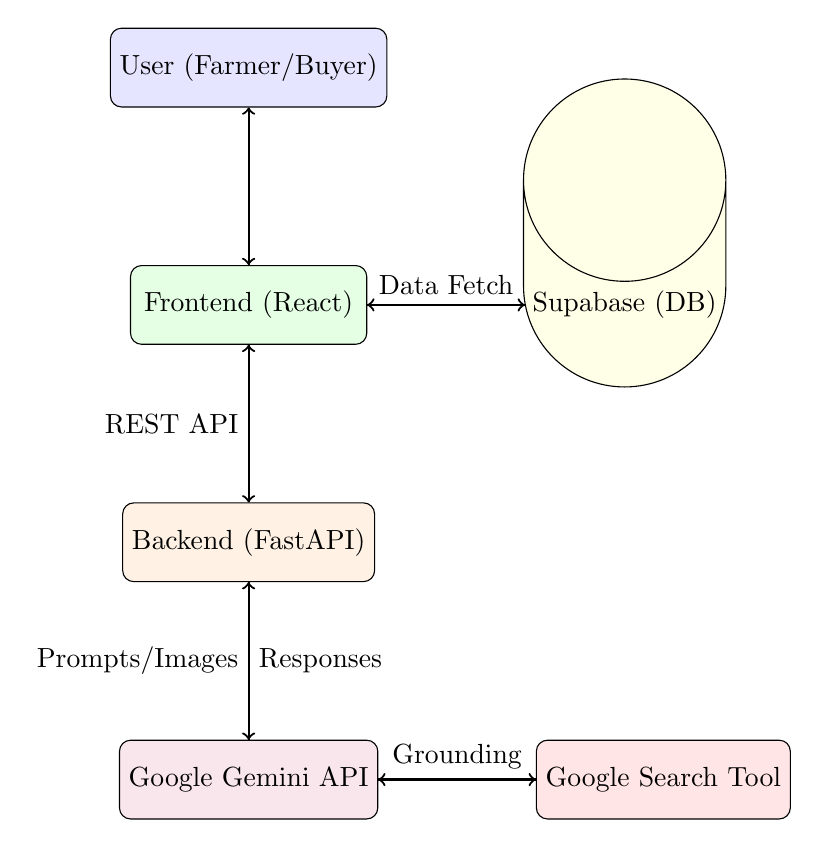
\begin{tikzpicture}[node distance=2cm]

% Nodes
\node (user) [rectangle, rounded corners, minimum width=3cm, minimum height=1cm, text centered, draw=black, fill=blue!10] {User (Farmer/Buyer)};

\node (frontend) [rectangle, rounded corners, minimum width=3cm, minimum height=1cm, text centered, draw=black, fill=green!10, below=of user] {Frontend (React)};

\node (backend) [rectangle, rounded corners, minimum width=3cm, minimum height=1cm, text centered, draw=black, fill=orange!10, below=of frontend] {Backend (FastAPI)};

\node (db) [cylinder, shape border rotate=90, draw, minimum width=2cm, minimum height=1.5cm, fill=yellow!10, right=of frontend] {Supabase (DB)};

\node (gemini) [rectangle, rounded corners, minimum width=3cm, minimum height=1cm, text centered, draw=black, fill=purple!10, below=of backend] {Google Gemini API};

\node (search) [rectangle, rounded corners, minimum width=3cm, minimum height=1cm, text centered, draw=black, fill=red!10, right=of gemini] {Google Search Tool};

% Arrows
\draw [->, thick] (user) -- (frontend);
\draw [->, thick] (frontend) -- (user);

\draw [->, thick] (frontend) -- node[anchor=east] {REST API} (backend);
\draw [->, thick] (backend) -- (frontend);

\draw [->, thick] (frontend) -- node[anchor=south] {Data Fetch} (db);
\draw [->, thick] (db) -- (frontend);

\draw [->, thick] (backend) -- node[anchor=east] {Prompts/Images} (gemini);
\draw [->, thick] (gemini) -- node[anchor=west] {Responses} (backend);

\draw [->, thick] (gemini) -- node[anchor=south] {Grounding} (search);
\draw [->, thick] (search) -- (gemini);

\end{tikzpicture}
\caption{System Architecture Flowchart}
\label{fig:arch}
\end{figure}

\section{AI Integration: The Role of Gemini}
We have strategically chosen Google's Gemini models for their multimodal capabilities and efficiency.

\subsection{Why Gemini? (Efficiency, Reliability, Trust)}
\subsubsection{1. Efficiency}
\begin{itemize}
    \item \textbf{Latency}: Gemini 1.5 Flash is optimized for high-frequency, low-latency tasks, making it ideal for real-time chatbots and price predictions.
    \item \textbf{Context Window}: The large context window allows us to pass detailed market reports or long government scheme documents for analysis without truncation.
    \item \textbf{Cost-Effectiveness}: Compared to training and hosting custom Large Language Models (LLMs) on GPU instances, using the Gemini API significantly reduces infrastructure costs.
\end{itemize}

\subsubsection{2. Reliability}
\begin{itemize}
    \item \textbf{Uptime}: Google's enterprise-grade infrastructure ensures high availability.
    \item \textbf{Multimodal Native}: Unlike models that patch vision onto text, Gemini is natively multimodal. This ensures superior performance in tasks like \textit{Quality Check}, where visual features (color, grain size) must be correlated with textual grading standards.
\end{itemize}

\subsubsection{3. Trustworthiness & Safety}
\begin{itemize}
    \item \textbf{Grounding with Google Search}: One of the biggest risks with LLMs is "hallucination." We mitigate this by using Gemini's \textbf{Grounding} feature. When a farmer asks about a subsidy, the model actively searches Google to verify facts before answering.
    \item \textbf{Citations}: The system provides source URLs (e.g., \texttt{agricoop.nic.in}) for every claim, allowing users to verify information independently.
    \item \textbf{Safety Filters}: Built-in safety settings prevent the generation of harmful or biased content.
\end{itemize}

\subsection{Core AI Modules}

\subsubsection{A. Multilingual Chatbot}
\textbf{Function}: Assists farmers with queries about schemes, weather, and farming techniques. \\
\textbf{Implementation}:
\begin{itemize}
    \item \textbf{Input}: Text (Hindi/English/Regional).
    \item \textbf{Process}: Intent detection classifies the query. If it requires external data (e.g., "latest MSP rates"), the \texttt{google\_search} tool is invoked.
    \item \textbf{Output}: A concise answer with source links.
\end{itemize}

\subsubsection{B. Visual Quality Analysis}
\textbf{Function}: Grades millet samples from photos. \\
\textbf{Implementation}:
\begin{itemize}
    \item \textbf{Input}: Image file (JPEG/PNG).
    \item \textbf{Process}: The image is encoded and sent to Gemini Vision. The prompt instructs the model to evaluate \textit{Grain Uniformity}, \textit{Color}, and \textit{Impurities}.
    \item \textbf{Output}: JSON object containing Quality Grade (A/B/C) and Moisture Estimate.
\end{itemize}

\subsubsection{C. Price Prediction Engine}
\textbf{Function}: Recommends fair selling prices. \\
\textbf{Implementation}:
\begin{itemize}
    \item \textbf{Input}: Millet Type, Location, Quality Grade.
    \item \textbf{Process}: The model acts as a market analyst, combining its internal knowledge base of agricultural economics with current market trends.
    \item \textbf{Output}: Recommended Price (INR/Quintal).
\end{itemize}

\section{Implementation Details}

\subsection{Backend Logic (FastAPI)}
The backend is designed for speed. Below is a snippet showing the hybrid intent detection logic:

\begin{lstlisting}[language=Python, caption=Hybrid Intent Detection in services.py]
async def generate_chat_response(query: str, context: str = ""):
    # 1. Intent Detection for Web Search
    SEARCH_KEYWORDS = ["scheme", "subsidy", "price", "market", "news"]
    needs_web_search = any(k in query.lower() for k in SEARCH_KEYWORDS)
    
    if needs_web_search:
        # Use Gemini with Google Search Tool
        model = genai.GenerativeModel('gemini-pro')
        response = model.generate_content(
            query, 
            tools=[Tool.google_search_retrieval]
        )
        return parse_search_response(response)
    else:
        # Fast path for general queries
        return simple_chat_response(query)
\end{lstlisting}

\subsection{Frontend Integration (React)}
The frontend communicates via a centralized API layer.

\begin{lstlisting}[language=JavaScript, caption=API Call for Price Prediction]
export const checkPrice = async (milletType, quality, location) => {
  const response = await fetch(`${AI_BASE_URL}/price-gemini`, {
    method: "POST",
    headers: {
      "Content-Type": "application/json",
      "X-API-Key": API_KEY,
    },
    body: JSON.stringify({ 
        millet_type: milletType, 
        quality_grade: quality, 
        location 
    }),
  });
  return response.json();
};
\end{lstlisting}

\section{Future Work}
To further enhance the platform, we propose the following roadmap:

\begin{enumerate}
    \item \textbf{Offline Capabilities with MarianMT}: 
    While Gemini is powerful, it requires internet. We plan to integrate \textbf{MarianMT} (Hugging Face) for on-device, offline translation. This will allow the app to function in remote areas with poor connectivity.
    
    \item \textbf{Voice-First Interface}:
    Integrating \textbf{OpenAI Whisper} or Google's Speech-to-Text to allow illiterate farmers to interact with the app purely via voice commands.
    
    \item \textbf{Blockchain Traceability}:
    Implementing a Hyperledger-based supply chain tracking system to issue immutable "Organic Certificates" for premium millets.
    
    \item \textbf{IoT Integration}:
    Connecting with IoT moisture sensors for more accurate (non-visual) quality testing.
\end{enumerate}

\section{Conclusion}
Shree Anna Connect demonstrates the transformative power of AI in agriculture. By leveraging Google Gemini's multimodal and grounding capabilities, we have built a system that is not only technologically advanced but also reliable and trustworthy. The architecture is robust, scalable, and ready for real-world deployment to help millions of millet farmers.

\section{Appendix: Anticipated Q\&A for Hackathon Judges}
This section addresses critical questions likely to be asked during the evaluation.

\subsection{Technical & Architectural Questions}

\textbf{Q1: Why did you use Gemini API instead of training your own model (e.g., YOLO, ResNet)?} \\
\textit{Answer:} 
\begin{itemize}
    \item \textbf{Multimodality}: Gemini is natively multimodal. It doesn't just "see" the image; it "reasons" about it. A standard YOLO model can detect a grain, but it cannot reason about "discoloration due to moisture" vs "natural color variant" as effectively without a massive labeled dataset.
    \item \textbf{Time-to-Market}: Training a robust agricultural model requires thousands of labeled images and weeks of fine-tuning. The API allowed us to build a production-ready prototype in 36 hours.
    \item \textbf{Maintenance}: Using a Foundation Model as a Service reduces the MLOps burden. We don't need to manage model drift or retraining pipelines.
\end{itemize}

\textbf{Q2: What happens if the internet connectivity is poor in rural areas?} \\
\textit{Answer:} 
\begin{itemize}
    \item \textbf{Current State}: The app is a Progressive Web App (PWA) that caches static content.
    \item \textbf{Future Roadmap}: We are integrating \textbf{MarianMT} (as detailed in Future Work) for on-device, offline translation. For critical features like price checking, we can implement SMS-based fallbacks.
\end{itemize}

\textbf{Q3: Is the system scalable?} \\
\textit{Answer:} Yes. The backend is stateless (FastAPI) and containerized (Docker). It can be horizontally scaled on any cloud platform (AWS/GCP). The database (Supabase) handles connection pooling automatically.

\subsection{Impact & Usability Questions}

\textbf{Q4: How will illiterate farmers use this app?} \\
\textit{Answer:} 
\begin{itemize}
    \item \textbf{Voice Interface}: We are adding Speech-to-Text (Whisper) so farmers can just "speak" their query.
    \item \textbf{Visual Navigation}: The UI relies heavily on icons and images rather than text.
    \item \textbf{Regional Languages}: The app already supports Hindi and English, with architecture ready for all 22 scheduled languages.
\end{itemize}

\textbf{Q5: How accurate is the Price Prediction?} \\
\textit{Answer:} It is an \textit{estimation} based on aggregated data. We use Gemini to parse unstructured news and market reports to find the latest trends. While not a replacement for a live trading terminal, it gives farmers a "fair range" to negotiate better, preventing exploitation.

\subsection{Business & Viability Questions}

\textbf{Q6: What is the revenue model?} \\
\textit{Answer:}
\begin{itemize}
    \item \textbf{Commission}: Small \% on successful B2B matches.
    \item \textbf{Premium Listings}: Certified organic farmers pay for "Verified" badges.
    \item \textbf{Data Insights}: Aggregated, anonymized crop data can be sold to agri-input companies and government agencies.
\end{itemize}

\textbf{Q7: How do you ensure the "Organic" tag is genuine?} \\
\textit{Answer:} Currently, it is self-declared but flagged for manual review. In the roadmap, we propose a \textbf{Blockchain-based Supply Chain} where certification bodies upload digital certificates that are immutable and verifiable via QR code.

\end{document}
